%ChSParams_Transmission.tex
%
%-------------------------------------------------------------------------------
\section{Scattering Transmission Parameters, $\matrixsymbol{T}$}
%-------------------------------------------------------------------------------
The scattering transmission matrix relates the normalized power waves in a form which computes the incident/reflected waves at port 1 as a function of those present at port 2:
\begin{equation}
	\left[\begin{IEEEeqnarraybox*}[][c]{,c,}
		b_{1}\\a_{1}%
	\end{IEEEeqnarraybox*}\right]
	=\left[\begin{IEEEeqnarraybox*}[][c]{,c/c,}
		t_{11}&t_{12}\\
		t_{21}&t_{22}%
	\end{IEEEeqnarraybox*}\right]
	\left[\begin{IEEEeqnarraybox*}[][c]{,c,}
		a_{2}\\b_{2}%
	\end{IEEEeqnarraybox*}\right]
	\textrm{.}
\end{equation}
%
The scattering transmission matrix is typically defined using $\matrixsymbol{T}$:
\begin{equation}
	\matrixsymbol{T}
	\defAs\left[\begin{IEEEeqnarraybox*}[][c]{,c/c,}
		t_{11}&t_{12}\\
		t_{21}&t_{22}%
	\end{IEEEeqnarraybox*}\right]
\end{equation}
%
Thus, the response for a cascade of networks can be computed from a simple matrix multiplication \emph{provided} the port 1 reference impedance of $\matrixsymbol{T}_{i+1}$ is equivalent to the port 2 reference impedance of $\matrixsymbol{T}_i$ (GENERATE FIGURE).
%
\subsubsection{Network Parameter Conversion ($\matrixsymbol{S}\Leftrightarrow\matrixsymbol{T}$)}
\par Taken from \cite{pr:Marks_1992} - have not confirmed whether correct - Derive?:
\begin{equation}
	\matrixsymbol{T}=\frac{1}{s_{21}}
	\left[\begin{IEEEeqnarraybox*}[][c]{,c"c,}
		s_{12}s_{21}-s_{11}s_{22}&s_{11}\\
		-s_{22}&1
	\end{IEEEeqnarraybox*}\right]
	\textrm{.}
\label{eq:StoT}%################################################################
\end{equation}
%
%------------------------------------------------------------------------------
\section{Cascade of 2 Transmission Line Segments}
\begin{figure}[!ht]
	\centering
	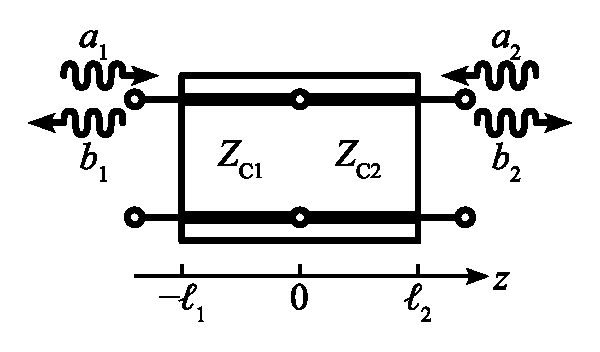
\includegraphics[scale=0.6]{ZCDiscontinuity}
	\caption{Cascaded transmission line segments.}
\label{fig:ZCDiscontinuity}%##################################################
\end{figure}
%
\par Consider the discontinuity in Fig.~\ref{fig:ZCDiscontinuity} formed by cascading transmission lines of different characteristic impedance values. Note that $z=0$ is now positionned at the discontinuity instead of the port interfaces. This notation will lead to a more elegant derivation of the network parameters.
%
\par Instead of using pseudo-waves, we will use traveling waves... TRY TO CONNECT SENTENCES. Next, consider the reference impedance of each port, $Z_\mathrm{01}$ and $Z_\mathrm{02}$ to respectively match these values, $Z_\mathrm{C1}$ and $Z_\mathrm{C2}$:
\begin{equation}
	Z_\mathrm{01}=Z_\mathrm{C1}
	\textrm{, and }
	Z_\mathrm{02}=Z_\mathrm{C2}
\label{eq:CascadedLines_Z0eqZC}%################################################
	\textrm{.}
\end{equation}
%
As a consequence, reflected waves will be fully absorbed by the port terminations during the conceptual $S$-parameter measurement that follows.  Given that the transmission lines are terminated with their respective $Z_{\mathrm{C}i}$, the forward \& reverse reflection coefficients at the interface of the discontinuity are given by (Fig.~\ref{fig:ZCDiscontinuity_Gamma}):
\begin{figure}[!ht]
	\centering
	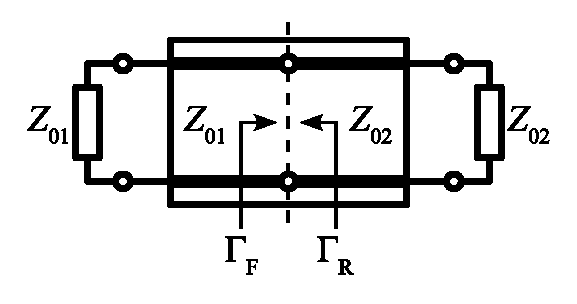
\includegraphics[scale=0.6]{ZCDiscontinuity_Gamma}
	\caption{Reflection coefficients at interface of perfectly terminated lines.}
\label{fig:ZCDiscontinuity_Gamma}%##################################################
\end{figure}
%
\begin{equation}
	\Gamma_\mathrm{F}= \frac{Z_\mathrm{02}-Z_\mathrm{01}}{Z_\mathrm{02}+Z_\mathrm{01}}
%\label{eq:ZPMatrixEquation}%###################################################
	\textrm{, and }
	\Gamma_\mathrm{R}= \frac{Z_\mathrm{01}-Z_\mathrm{02}}{Z_\mathrm{01}+Z_\mathrm{02}}
	\textrm{.}
\end{equation}
%
where
\begin{itemize}%[\setlabelwidth{}]
	\item[]Subscripts ``F", and ``R" identify quantities as ``forward" or ``reverse" reflection coefficients, respectively.
\end{itemize}
%
\subsubsection{Forward Transmission/Reflection}
\begin{figure}[!ht]
	\centering
	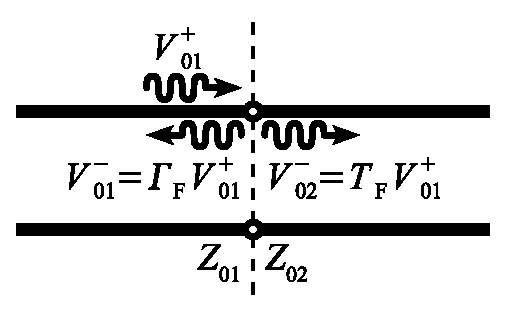
\includegraphics[scale=0.6]{ZCDiscontinuity_Forward}
	\caption{Forward transmission/reflection at the discontinuity.}
\label{fig:ZCDiscontinuity_Forward}%##################################################
\end{figure}
%
Next, consider the forward transmission/reflection (excitation at port 1 only) of a wave through the discontinuity (Fig.~\ref{fig:ZCDiscontinuity_Forward}). If $V^+_{01}$ defines the incident wave phasor at the discontinuity itself, position-dependent expressions for the incident, reflected and transmitted wave phasors are given by:
\begin{IEEEeqnarray}{rl}
	V_\mathrm{F}^\mathrm{I}(z)
		&{}=V^+_{01}e^{-{\gamma_1}z}
\label{eq:IncVoltAtZCDisc}%#####################################################
		\textrm{,}\\
	V_\mathrm{F}^\mathrm{R}(z)
		&{}=V^-_{01}e^{{\gamma_1}z}={\Gamma_\mathrm{F}}V^+_{01}e^{{\gamma_1}z}
\label{eq:ReflVoltAtZCDisc}%####################################################
		\textrm{,}\\\textrm{and }
	V_\mathrm{F}^\mathrm{T}(z)
		&{}={V^-_{02}}e^{{\gamma_2}z}=(V^+_{01}+V^-_{01})e^{-{\gamma_2}z}
		=(1+\Gamma_\mathrm{F})V^+_{01}e^{-{\gamma_2}z}
\label{eq:TransVoltAtZCDisc}%###################################################
	\textrm{.}
\end{IEEEeqnarray}
%
Thus, the forward transmission coefficient is defined as $T{\equiv}1+\Gamma_\mathrm{F}$.
%
\subsubsection{Power Conservation at the Discontinuity}
\par Verify power conservation.  Was not able to do so, but should work as follows.  Using \eqref{eq:IncTransReflPower} at the discontinuity ($z=0$):
\begin{IEEEeqnarray*}{rl}
	\textrm{incident power}
		&{}=\textrm{transmitted power}+\textrm{reflected power}\IEEEyesnumber\\
	P^\mathrm{I}_F
		&{}=P^\mathrm{T}_F+P^\mathrm{R}_F\\
	\frac{1}{2}\frac{V^\mathrm{I}_F\cdot V^{\mathrm{I}*}_F}{\realS{Z_{01}}}
		&{}=\frac{1}{2}\frac{V^\mathrm{T}_F\cdot V^{\mathrm{T}*}_F}{\realS{Z_{02}}}
		+\frac{1}{2}\frac{V^\mathrm{R}_F\cdot V^{\mathrm{R}*}_F}{\realS{Z_{01}}}\\
	\frac{1}{\realS{Z_{01}}}
			&{}=\frac{(1+\Gamma_\mathrm{F})\cdot(1+\Gamma_\mathrm{F})^*}{\realS{Z_{02}}}
			+\frac{\Gamma_\mathrm{F}\cdot \Gamma_\mathrm{F}^*}{\realS{Z_{01}}}
	\textrm{.}\IEEEyesnumber
\end{IEEEeqnarray*}
%
\subsubsection{Scattering Parameters}
\par The forward scattering parameters of the network in Fig.~\ref{fig:ZCDiscontinuity} can therefore be computed from the phasor values at the port interfaces:
\begin{IEEEeqnarray*}{l}
\EAtwocols
	{s_{11}}{
		{}=\left.\frac{b_1}{a_1}\right|_{a_2=0}
		=\frac{V_\mathrm{F}^\mathrm{R}(-\ell_1)/\sqrt{Z_{01}}}{V_\mathrm{F}^\mathrm{I}(-\ell_1)/\sqrt{Z_{01}}}
	}{s_{21}}{
		{}=\left.\frac{b_2}{a_1}\right|_{a_2=0}
		=\frac{V_\mathrm{F}^\mathrm{T}(\ell_2)/\sqrt{Z_{02}}}{V_\mathrm{F}^\mathrm{I}(-\ell_1)/\sqrt{Z_{01}}}
	}
\\\EAtwocols
	{\therefore s_{11}}{
		{}=\Gamma_\mathrm{F}e^{-2{\gamma_1}\ell_1}
	}{\therefore s_{21}}{
		{}=\frac{\sqrt{Z_{01}}}{\sqrt{Z_{02}}}(1+\Gamma_\mathrm{F})e^{-({\gamma_1}\ell_1+{\gamma_2}\ell_2)}
		\textrm{.}
	}\IEEEyesnumber
\end{IEEEeqnarray*}
%
\par By symmetry, and because $\Gamma_\mathrm{R}=-\Gamma_\mathrm{F}$, the reverse transmission coefficients are given by:
\begin{IEEEeqnarray*}{l}
\EAtwocols
	{s_{22}}{
		{}=\left.\frac{b_2}{a_2}\right|_{a_1=0}
		=\Gamma_\mathrm{R}e^{-2{\gamma_2}\ell_2}
	}{s_{12}}{
		{}=\left.\frac{b_1}{a_2}\right|_{a_1=0}
		=\frac{\sqrt{Z_{02}}}{\sqrt{Z_{01}}}(1+\Gamma_\mathrm{R})e^{-({\gamma_1}\ell_1+{\gamma_2}\ell_2)}
	}
\\\EAtwocols
	{\therefore s_{22}}{
		{}=-\Gamma_\mathrm{F}e^{-2{\gamma_2}\ell_2}
	}{\therefore s_{12}}{
		{}=\frac{\sqrt{Z_{02}}}{\sqrt{Z_{01}}}(1-\Gamma_\mathrm{F})e^{-({\gamma_1}\ell_1+{\gamma_2}\ell_2)}
		\textrm{.}
	}\IEEEyesnumber
\end{IEEEeqnarray*}
%
%------------------------------------------------------------------------------
\section{$S$-Parameter Reference Impedance Transformer}
\par The result of matching the $S$-parameter reference impedances of the cascaded transmission line segments to their respective line impedances in \eqref{eq:CascadedLines_Z0eqZC} is to reference the associated \emph{power waves} ($a_1$, $b_1$, $a_2$, and $b_2$) to those same impedances. This property can easily be leveraged to perform a transformation of reference impedances.
%
\par Consider a transmitter designed to drive a line of $Z_\mathrm{C}=Z_{0\mathrm{TX}}$. The simulated linear $S$-parameter model of the transmitter would typically be referenced to a (often real) frequency independant impedance, $Z_{0\mathrm{S}}$.  Conceptually, the output can be connected to pair of cascaded transmission lines with arbitrary characteristic impedances.  However, if the $Z_{01}$ connected to the driver output matches $Z_{0\mathrm{S}}$, the network cascade is more readily computed from the two $\matrixsymbol{T}$ matrices. Furthermore, if the length of both line segments are set to zero, the cascade of lines degenerates into an ideal thru, thus behaving as a perfect $Z_{01}:Z_{02}$ transformer. If $Z_{02}$ is then chosen to correspond to $Z_{0\mathrm{TX}}$, the resulting $\matrixsymbol{T}$-matrix will therefore be referenced to the physical \emph{traveling} waves $a^{'}_{\mathrm{TX}}$ \& $b^{'}_{\mathrm{TX}}$ GENERATE FIGURE.
%
\par The $\matrixsymbol{T}$-matrix of the impedance transformer is therefore obtained by substituting REF EQ for $\ell_1=\ell_2=0$ in \eqref{eq:StoT}:
\begin{IEEEeqnarray*}{l}
\EAtwocols
	{t_{11}}{{}=\left.\frac{s_{12}s_{21}-s_{11}s_{22}}{s_{21}}\right|_{\ell_1=\ell_2=0}}
	{t_{12}}{{}=\left.\frac{s_{11}}{s_{21}}\right|_{\ell_1=\ell_2=0}}
\\\EAtwocols
	{t_{21}}{{}=\left.\frac{-s_{22}}{s_{21}}\right|_{\ell_1=\ell_2=0}}
	{t_{22}}{{}=\left.\frac{1}{s_{21}}\right|_{\ell_1=\ell_2=0}\textrm{.}}
\end{IEEEeqnarray*}
%
Which yields:
\begin{equation}
	\matrixsymbol{T}=\frac{1}{1+\Gamma_\mathrm{F}}
	\frac{\sqrt{Z_{02}}}{\sqrt{Z_{01}}}
	\left[\begin{IEEEeqnarraybox*}[][c]{,c/c,}
		1&\Gamma_\mathrm{F}\\
		\Gamma_\mathrm{F}&1
	\end{IEEEeqnarraybox*}\right]
	\textrm{.}
%\label{eq:StoT}%################################################################
\end{equation}
%
\par Another interresting form is obtained by noting that $1+\Gamma_\mathrm{F}=\frac{2Z_{02}}{Z_{02}+Z_{01}}$:
\begin{equation}
	\matrixsymbol{T}=\frac{1}{2Z_{02}}
	\frac{\sqrt{Z_{02}}}{\sqrt{Z_{01}}}
	\left[\begin{IEEEeqnarraybox*}[][c]{,c/c,}
		Z_{02}+Z_{01}&Z_{02}-Z_{01}\\
		Z_{02}-Z_{01}&Z_{02}+Z_{01}
	\end{IEEEeqnarraybox*}\right]
	\textrm{.}
%\label{eq:StoT}%################################################################
\end{equation}
%
\par Note: This does not match eq.\ 79 of \cite{pr:Marks_1992}.  One of the reasons may have something to do with the fact the $Q^{nm}$ matrix is defined with $a_n$ \& $b_n$ rows reversed.  Note that eq.\ 79 also an extra term,  $\left|Z_{02}/Z_{01}\right|$. If we let $\sqrt{Z_{0i}}\defAs r_ie^{j\theta_i}$, we get:
%
\begin{IEEEeqnarray*}{rl}
	\left|\frac{Z_{02}}{Z_{01}}\right|
	&=\left|\frac{(r_2e^{j\theta_2})^2}{(r_1e^{j\theta_1})^2}\right|
	=\left|\frac{r^2_2e^{j2\theta_2}}{r^2_1e^{j2\theta_1}}\right|
	=\frac{r^2_2}{r^2_1}
	\textrm{.}
\end{IEEEeqnarray*}
\par I cannot explain this discrepancy.
%
%Last line